\documentclass[12pt, a4paper]{article}

\usepackage[top=2.5cm, bottom=2.5cm, left=2.5cm, right=2.5cm]{geometry}
\usepackage{graphicx}
\graphicspath{{plots/}}
\usepackage{amsmath, amssymb, amsfonts}
\usepackage{caption}
\usepackage{subcaption}
\usepackage{booktabs}
\usepackage{array}
\usepackage{float}
\usepackage{hyperref}
\usepackage{listings}
\usepackage{xcolor}
\usepackage{fancyhdr}
\usepackage{titlesec}
\usepackage{tocloft}
\usepackage{setspace}
\usepackage{cite}
\usepackage{url}
\usepackage{parskip}

\lstset{
  language=Python,
  basicstyle=\ttfamily\footnotesize,
  keywordstyle=\color{blue}\bfseries,
  commentstyle=\color{gray}\itshape,
  stringstyle=\color{red!70!black},
  numberstyle=\tiny\color{gray},
  numbers=left,
  stepnumber=1,
  numbersep=8pt,
  breaklines=true,
  breakatwhitespace=false,
  frame=single,
  rulecolor=\color{black!30},
  backgroundcolor=\color{gray!5},
  captionpos=b,
  tabsize=4,
  showstringspaces=false,
  xleftmargin=15pt,
  xrightmargin=5pt
}

\pagestyle{fancy}
\fancyhf{}
\fancyhead[L]{\small EE 325 Digital Signal Processing}
\fancyhead[R]{\small Laboratory Report 01}
\fancyfoot[C]{\thepage}
\renewcommand{\headrulewidth}{0.4pt}
\setlength{\headheight}{14pt}

\begin{document}
\pagenumbering{gobble}
\begin{titlepage}
  \begin{center}
    \vspace*{1cm}
    {\large \textbf{UNIVERSITY OF PERADENIYA}} \\[0.3cm]
    {\large Faculty of Engineering} \\[0.3cm]
    {\large Department of Electrical and Electronic Engineering} \\[2cm]

    \rule{\linewidth}{0.5mm} \\[0.4cm]
    {\LARGE \textbf{EE 325: Digital Signal Processing}} \\[0.3cm]
    {\Large \textbf{Laboratory Report 01}} \\[0.3cm]
    {\Large Frequency Estimation Using Spectral Analysis Methods} \\[0.2cm]
    \rule{\linewidth}{0.5mm} \\[2cm]

    \begin{tabular}{ll}
      \textbf{Student Name:}    & Dineth Perera \\[0.2cm]
      \textbf{Registration No:} & E/21/291 \\[0.2cm]
      \textbf{Degree Program:}  & B.Sc. Engineering (Electrical \& Electronic) \\[0.2cm]
      \textbf{Academic Year:}   & 2024/2025 \\[0.2cm]
      \textbf{Date Submitted:}  & \today \\[0.2cm]
    \end{tabular}

    \vfill
    {\small Department of Electrical and Electronic Engineering \\
    University of Peradeniya, Peradeniya 20400, Sri Lanka}
  \end{center}
\end{titlepage}

\clearpage
\pagenumbering{arabic}
\tableofcontents
\newpage

\section{Introduction}
Frequency estimation is a core digital signal processing task because engineering measurements often contain multiple deterministic tones embedded in stochastic disturbances. In power systems, communications, rotating machinery diagnostics, and radar front-ends, the analyst must decide whether a signal is stationary, how many spectral components are present, and which estimation method is appropriate under noise and finite-data limitations \cite{oppenheim2010, proakis2007}. This laboratory studies that problem by comparing classical Fourier analysis, time-frequency analysis, correlation-based estimators, and high-resolution subspace methods on two signals constructed from the student-specific parameters for E/21/291.

For this registration number, the extracted digits are $a=2$, $b=9$, and $c=1$, which yield the sinusoidal frequencies $f_1=12$ Hz, $f_2=39$ Hz, and $f_3=71$ Hz. The analysis sequence in this report follows the laboratory tasks directly: time-domain inspection, histograms, the DFT, spectrograms, autocorrelation, periodogram formation, Pisarenko-based autocorrelation matrix sizing, MUSIC pseudo-spectrum estimation, and autoregressive spectrum estimation \cite{mitra2011, stoica2005}. The goal is not only to estimate the frequencies but also to evaluate what each method reveals about stationary and non-stationary signals.

\section{Signal Parameters and Construction}
The student parameters are derived directly from the registration number:
\begin{equation}
E/21/291 \Rightarrow a=2,\; b=9,\; c=1.
\end{equation}
Therefore, the three sinusoidal frequencies are
\begin{equation}
f_1 = 10 + a = 12\ \text{Hz}, \qquad
f_2 = 30 + b = 39\ \text{Hz}, \qquad
f_3 = 70 + c = 71\ \text{Hz}.
\end{equation}
The additive noise sequence is zero-mean unit-variance Gaussian noise,
\begin{equation}
\nu[n] \sim \mathcal{N}(0,1).
\end{equation}
With sampling frequency $F_s = 200$ Sa/s and duration $0 \le t \le 100$ s, the uniformly sampled time vector contains
\begin{equation}
N = 100 \times 200 + 1 = 20001
\end{equation}
samples. The two laboratory signals are therefore
\begin{equation}
x_1(t) = \sin(2\pi \cdot 12\, t) + \cos(2\pi \cdot 39\, t) + \sin(2\pi \cdot 71\, t) + \nu(t),
\end{equation}
and
\begin{equation}
x_2(t) = \sin\!\left(20\pi t + 2\pi \frac{t^2}{150}\right) + \nu(t).
\end{equation}
The first signal is stationary apart from the additive noise, whereas the second is a chirp whose instantaneous frequency increases linearly with time. These two cases make it possible to compare estimators intended for stationary spectra against a non-stationary waveform \cite{oppenheim2010, proakis2007}.

\section{Task 1 and Task 2: Time-Domain Signals and Histograms}
The first task was to construct the signals and inspect them directly in time. As shown in Fig.~\ref{fig:signals_td}, the first 2 s of each signal were plotted because the full 100 s record compresses the oscillations too strongly for visual interpretation.
\begin{figure}[H]
  \centering
  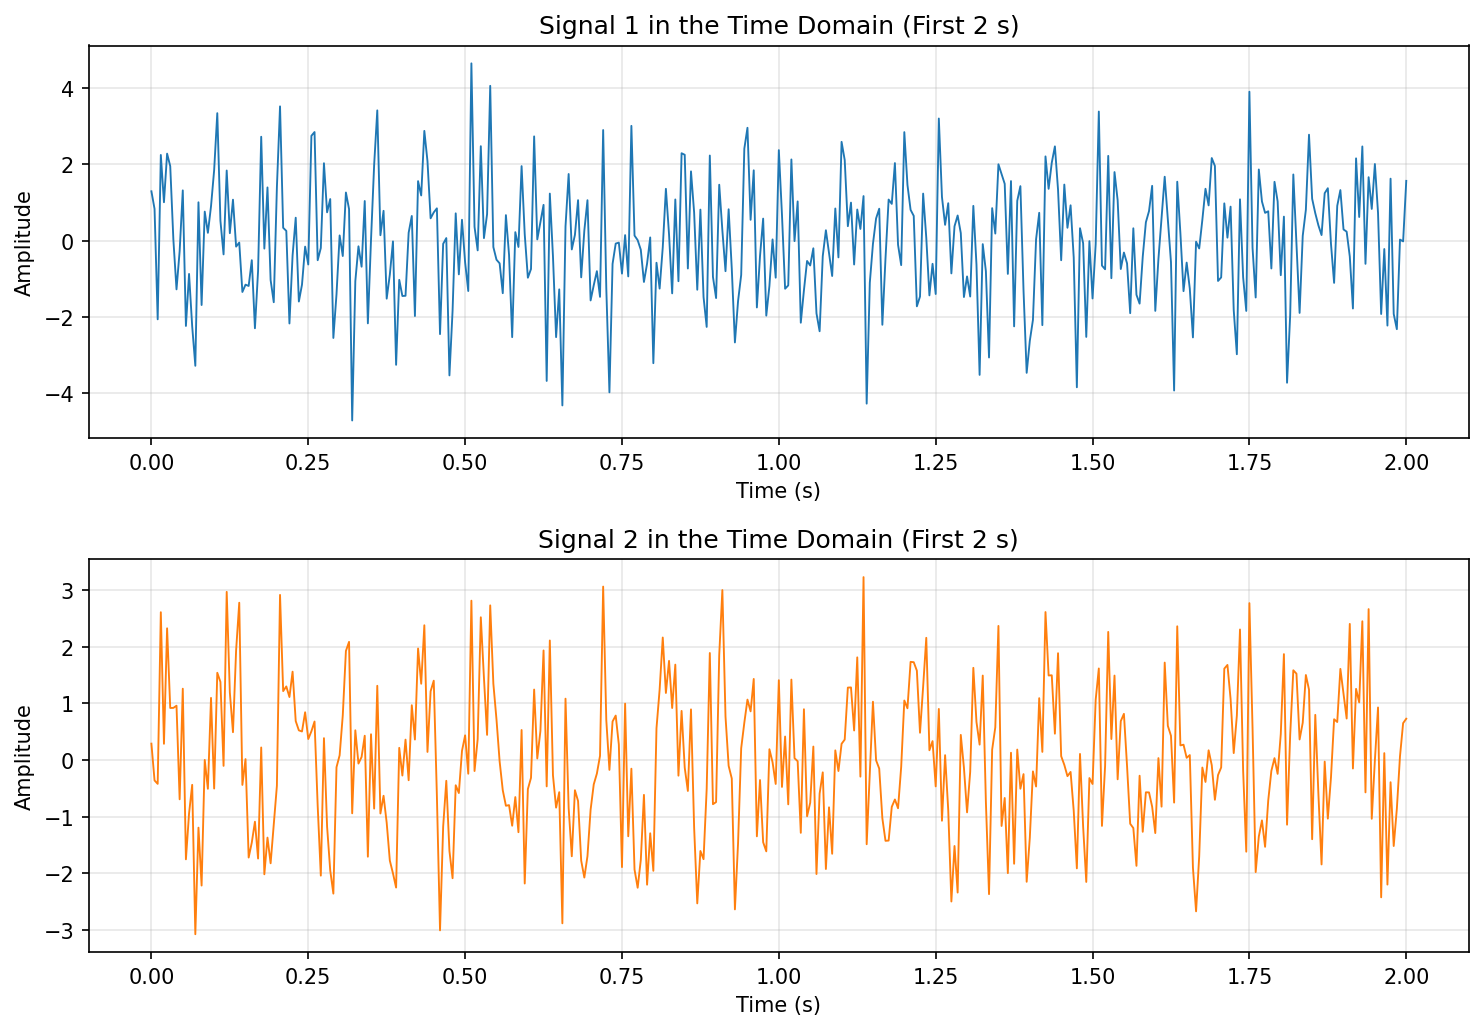
\includegraphics[width=0.88\textwidth]{lab01_fig01_signals.png}
  \caption{Time-domain views of Signal 1 and Signal 2 over the first 2 s.}
  \label{fig:signals_td}
\end{figure}

Figure~\ref{fig:signals_td} shows that Signal 1 appears highly irregular in the time domain because the three deterministic tones are superposed and then perturbed by Gaussian noise. The individual 12 Hz, 39 Hz, and 71 Hz components are therefore not directly separable from the waveform itself. Signal 2 has nearly constant amplitude envelope, but the oscillation density increases with time, which is a visual signature of chirp behavior.

The histogram requirement is satisfied in Fig.~\ref{fig:histograms}. The histogram of Signal 1 is broader and more bell-shaped because it is the sum of several independent contributions, while the histogram of Signal 2 remains centered but reflects the sinusoidal chirp plus the same noise sequence.
\begin{figure}[H]
  \centering
  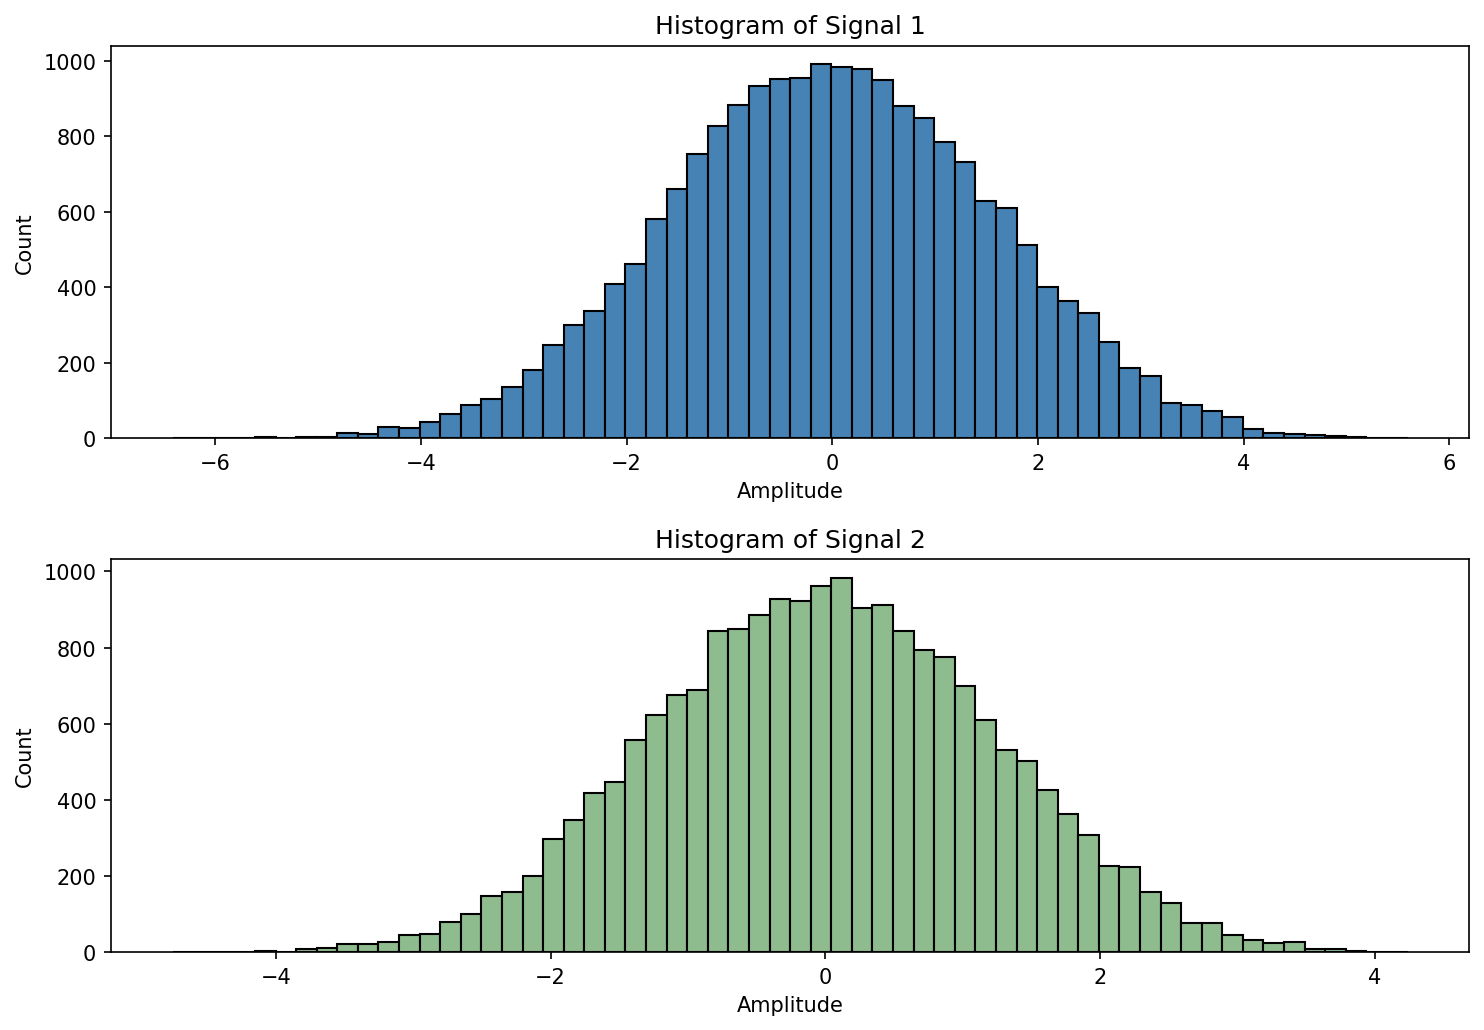
\includegraphics[width=0.88\textwidth]{lab01_fig02_histograms.png}
  \caption{Amplitude histograms of Signal 1 and Signal 2.}
  \label{fig:histograms}
\end{figure}

Signal 1 approaches a Gaussian-like distribution because the three deterministic terms and the random noise collectively increase the central concentration of the sample amplitudes. Signal 2 is somewhat flatter because the chirp traverses phase uniformly over the long record, yet the noise still broadens the distribution around zero.

\section{Task 3: Discrete Fourier Transform Analysis}
The next task was to compute the DFT and identify the dominant frequency components. The one-sided magnitude spectra obtained with \texttt{scipy.fft.fft} are shown in Fig.~\ref{fig:dft}.
\begin{figure}[H]
  \centering
  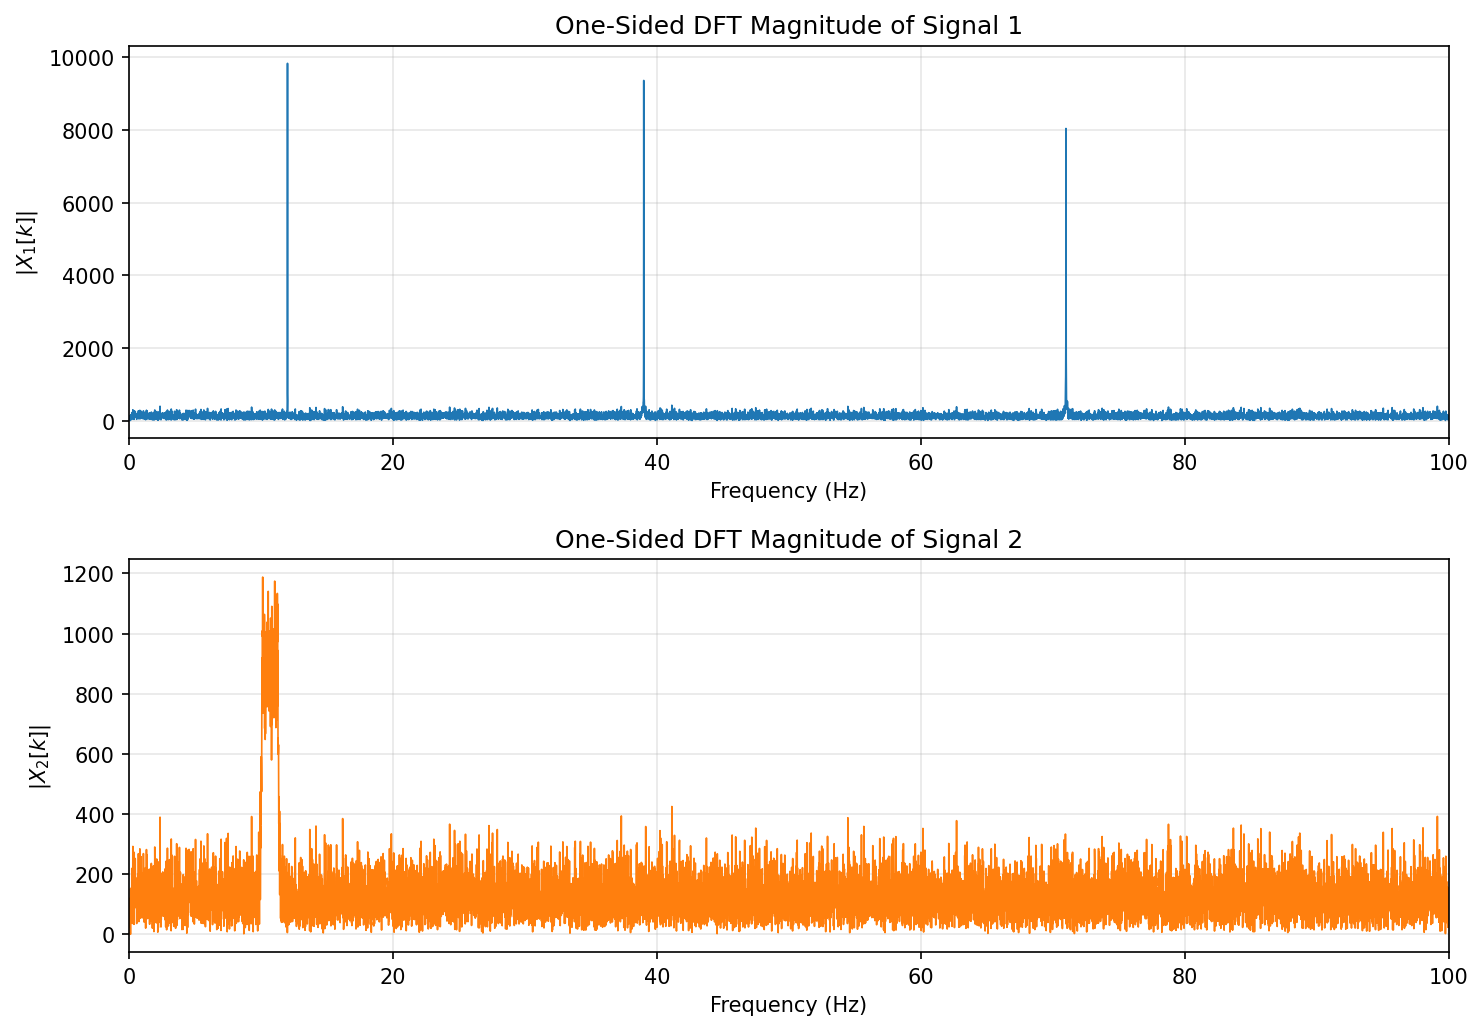
\includegraphics[width=0.88\textwidth]{lab01_fig03_dft.png}
  \caption{One-sided DFT magnitude spectra of Signal 1 and Signal 2.}
  \label{fig:dft}
\end{figure}

For the sampled record length $N=20001$, the frequency resolution is
\begin{equation}
\Delta f = \frac{F_s}{N} = \frac{200}{20001} \approx 0.0099995\ \text{Hz}.
\end{equation}
That fine grid makes the three deterministic tones easy to identify in Signal 1. The measured peak locations from the DFT are listed in Table~\ref{tab:dftresults}. These estimates are all within about $0.004$ Hz of the true frequencies, which is consistent with the available DFT bin spacing and the slight leakage associated with the finite data record \cite{oppenheim2010}.

The frequency comparison is summarized in Table~\ref{tab:dftresults}.
\begin{table}[H]
  \centering
  \caption{DFT-based frequency estimates for Signal 1.}
  \label{tab:dftresults}
  \begin{tabular}{ccc}
    \toprule
    True Frequency (Hz) & Estimated Frequency (Hz) & Error (Hz) \\
    \midrule
    12.000 & 11.9994 & 0.0006 \\
    39.000 & 38.9981 & 0.0019 \\
    71.000 & 70.9965 & 0.0035 \\
    \bottomrule
  \end{tabular}
\end{table}

The DFT of Signal 2 in Fig.~\ref{fig:dft} does not show isolated narrow spectral lines. Instead, the energy is smeared across a frequency range because a chirp is non-stationary: its instantaneous frequency changes during the observation interval, so the transform of the full record spreads energy over the visited band rather than concentrating it at fixed sinusoidal frequencies \cite{mitra2011}.

\section{Task 4: Spectrogram Analysis}
The fourth task was to analyze both signals using a short-time Fourier representation. The spectrograms in Fig.~\ref{fig:spectrograms} were computed with \texttt{nperseg}=512 and \texttt{noverlap}=384. This corresponds to a 2.56 s analysis window and 75\% overlap, which gives moderate frequency resolution while retaining enough time localization to track the chirp trajectory \cite{welch1967}.
\begin{figure}[H]
  \centering
  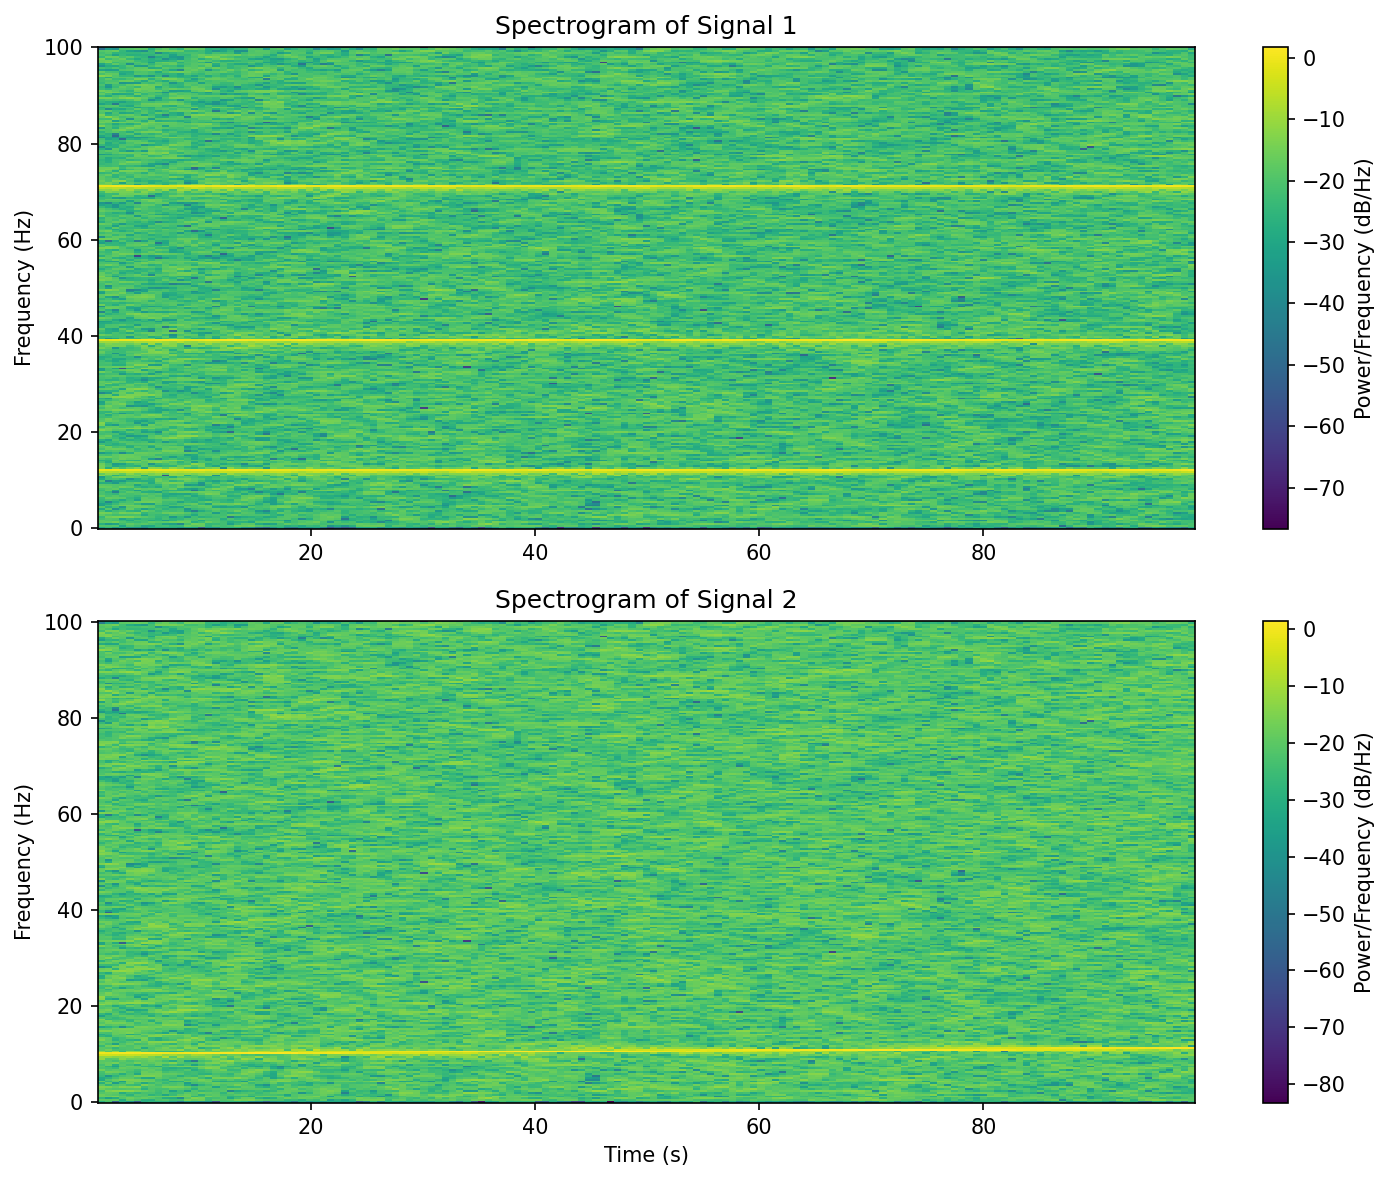
\includegraphics[width=0.88\textwidth]{lab01_fig04_spectrogram.png}
  \caption{Spectrograms of Signal 1 and Signal 2.}
  \label{fig:spectrograms}
\end{figure}

Figure~\ref{fig:spectrograms} shows three persistent horizontal bands in Signal 1 at approximately 12 Hz, 39 Hz, and 71 Hz, confirming that those components are stationary throughout the record. In contrast, Signal 2 exhibits a clear diagonal ridge: the energy starts at low frequency and rises with time, exactly as expected from a chirp. This is the strongest evidence in the report that Signal 2 is not stationary, because the spectral content is explicitly time-varying \cite{welch1967}.

\section{Task 5 and Task 6: Autocorrelation Analysis}
Tasks 5 and 6 required both the built-in autocorrelation estimator and the power-signal approximation estimator. The biased built-in estimator used in the code is
\begin{equation}
\hat{r}_{xx,\mathrm{built}}[\ell] = \frac{1}{N}\sum_{n} x[n]x[n-\ell],
\end{equation}
while the power-signal approximation requested in the laboratory sheet is
\begin{equation}
\hat{r}_{xx}[\ell] = \frac{1}{N-|\ell|}\sum_{n=0}^{N-|\ell|-1} x[n+|\ell|]x[n].
\end{equation}
The two Signal 1 autocorrelation plots are shown in Fig.~\ref{fig:acf1}.
\begin{figure}[H]
  \centering
  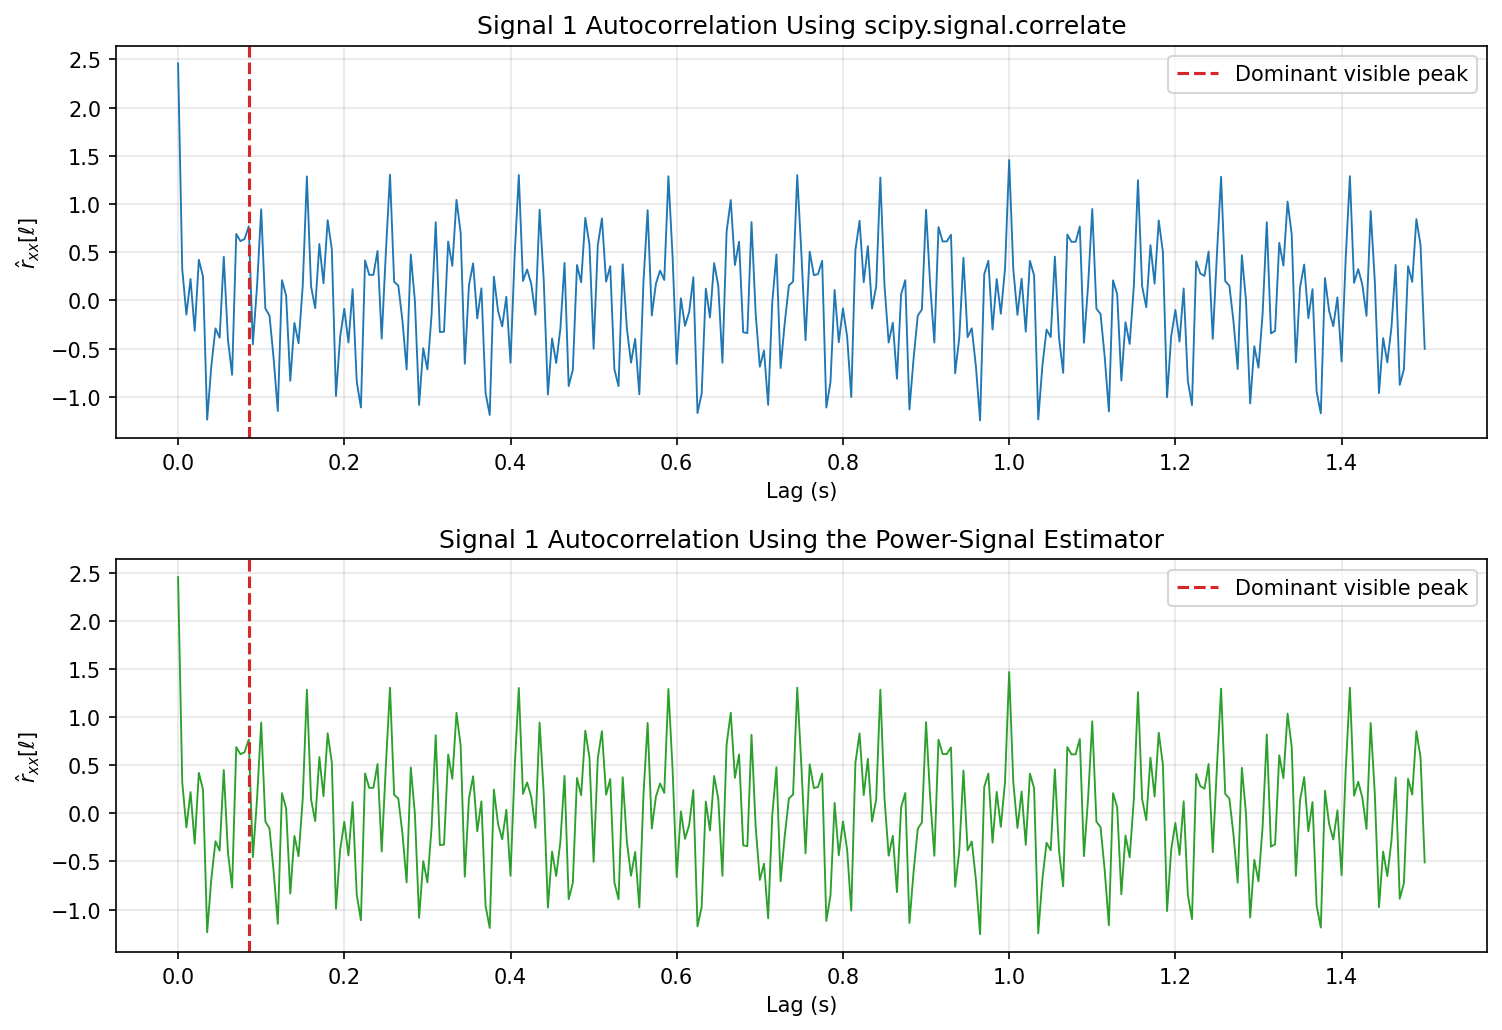
\includegraphics[width=0.88\textwidth]{lab01_fig05_autocorr_s1.png}
  \caption{Signal 1 autocorrelation using the built-in estimator and the power-signal estimator.}
  \label{fig:acf1}
\end{figure}

Signal 1 has an exact common period given by the reciprocal of the greatest common divisor of its component frequencies:
\begin{equation}
T_0 = \frac{1}{\gcd(12,39,71)} = 1\ \text{s}.
\end{equation}
However, the strongest visible local periodicity near the origin occurs at about 0.085 s in Fig.~\ref{fig:acf1}, which is close to $1/12 \approx 0.0833$ s. This occurs because the lowest-frequency sinusoid contributes the most easily visible short-lag oscillatory structure. The power-signal estimator preserves the correlation level at larger lags more faithfully than the built-in $1/N$ normalization because it compensates for the decreasing number of overlapping samples \cite{oppenheim2010, proakis2007}.

The corresponding chirp autocorrelation plots are shown in Fig.~\ref{fig:acf2}.
\begin{figure}[H]
  \centering
  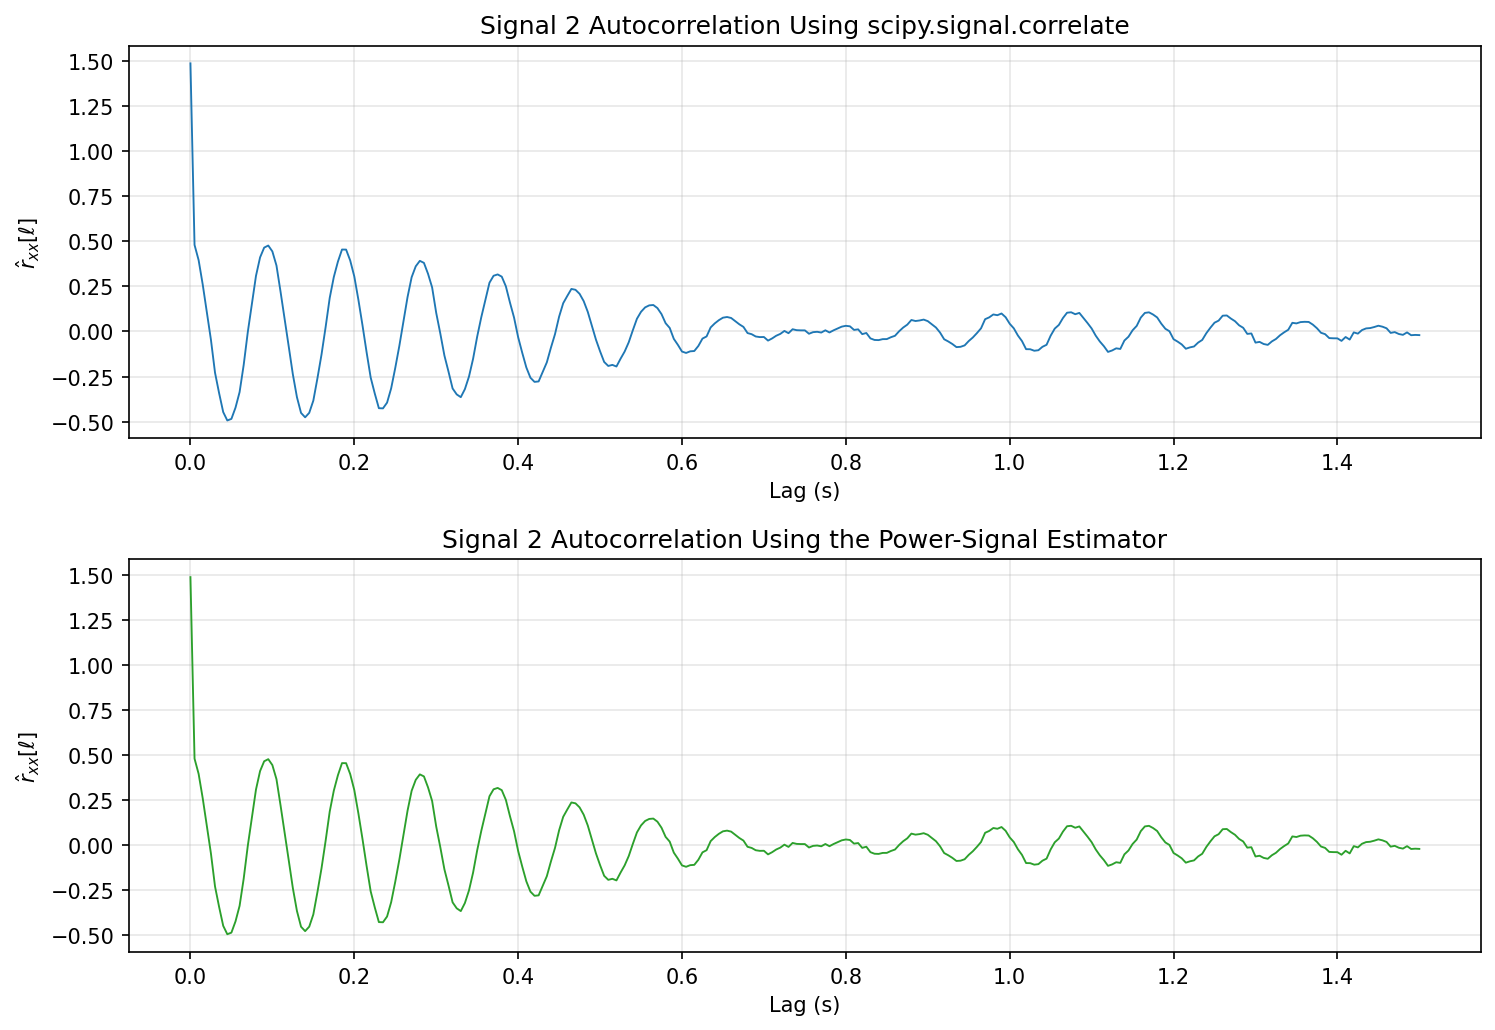
\includegraphics[width=0.88\textwidth]{lab01_fig06_autocorr_s2.png}
  \caption{Signal 2 autocorrelation using the built-in estimator and the power-signal estimator.}
  \label{fig:acf2}
\end{figure}

For Signal 2, period identification is not meaningful in the same way because the signal is non-stationary. Figure~\ref{fig:acf2} shows a rapidly decaying and distorted correlation pattern rather than a clean repetitive sequence of peaks. This is expected: autocorrelation is best interpreted as a periodicity indicator when the waveform statistics do not vary strongly with time.

\section{Task 7: Periodogram}
Task 7 required the periodogram to be formed as the DFT of the full autocorrelation sequence rather than by calling \texttt{periodogram()} directly. The resulting one-sided linear-scale plots are shown in Fig.~\ref{fig:periodogram}.
\begin{figure}[H]
  \centering
  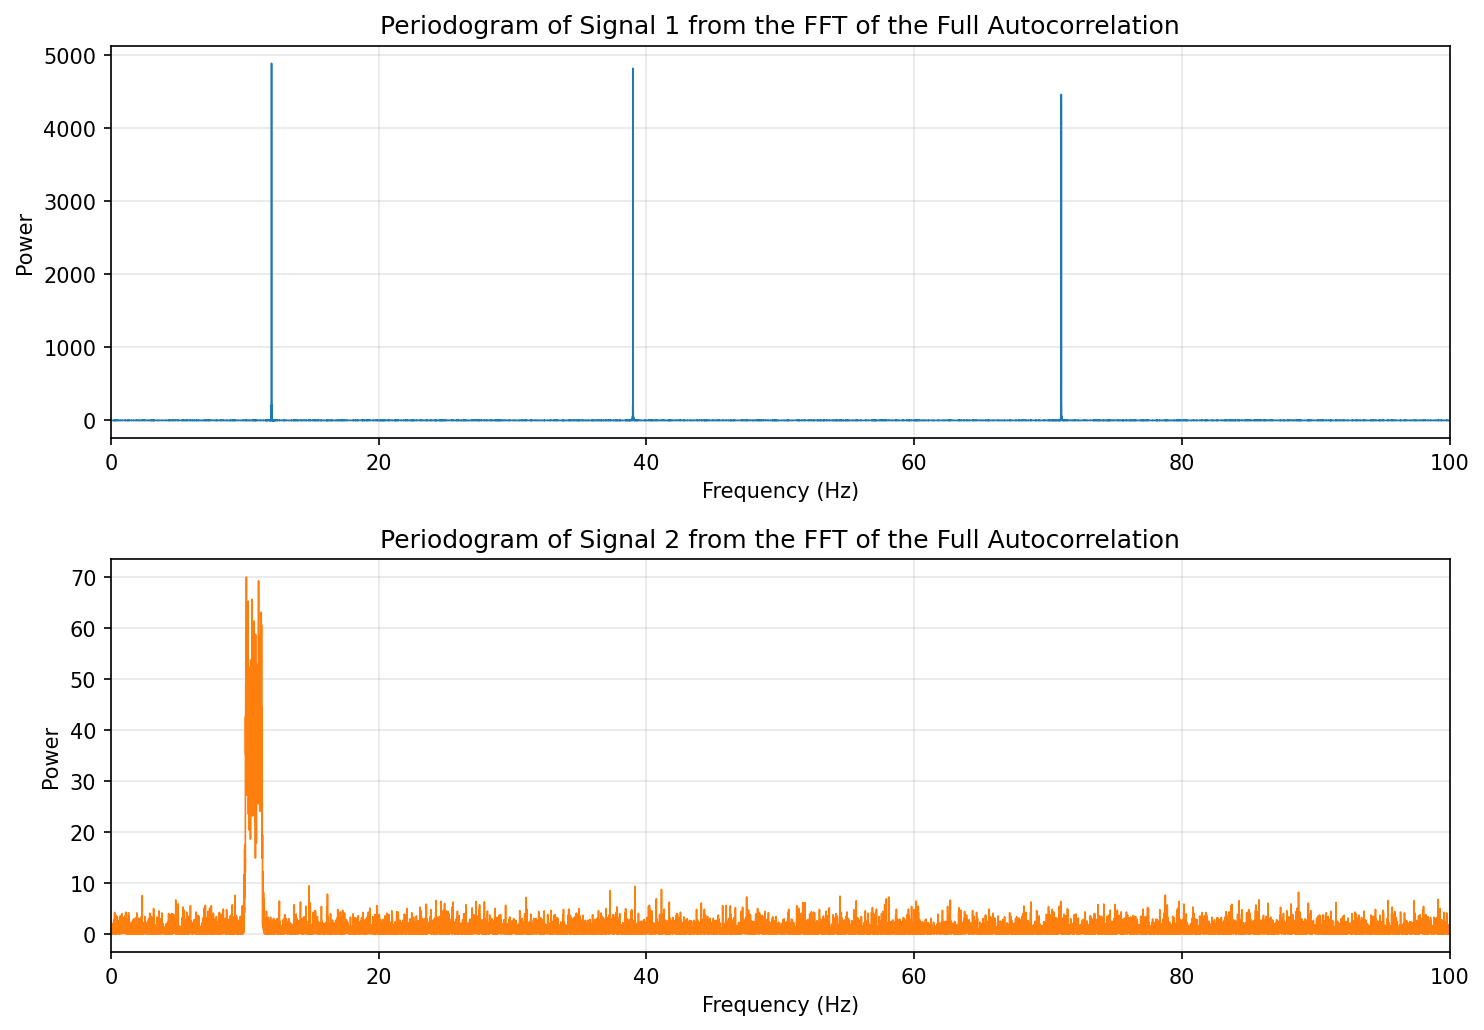
\includegraphics[width=0.88\textwidth]{lab01_fig07_periodogram.png}
  \caption{Periodograms of Signal 1 and Signal 2 formed from the FFT of the full autocorrelation sequence.}
  \label{fig:periodogram}
\end{figure}

The periodogram relationship used here is
\begin{equation}
P_{xx}(f) = \left| \mathcal{F}\left\{\hat{r}_{xx}[\ell]\right\} \right|.
\end{equation}
For Signal 1, the periodogram peaks occur at 11.9997 Hz, 38.9990 Hz, and 70.9982 Hz, which are essentially identical to the DFT-based estimates in Table~\ref{tab:dftresults}. Compared with the raw DFT, the periodogram view emphasizes the power-distribution interpretation of the same spectral content \cite{welch1967}. For the chirp, the energy remains broadened because the underlying signal is not stationary, so a single global spectrum still aggregates many instantaneous frequencies.

\section{Task 8: Autocorrelation Matrix Size for PHD}
Signal 1 contains $K=3$ real sinusoidal tones. Each real sinusoid corresponds to a pair of complex exponentials at $\pm \omega$, so the total number of spectral components is
\begin{equation}
p = 2K = 6.
\end{equation}
Therefore, the Pisarenko harmonic decomposition requires an autocorrelation matrix of size
\begin{equation}
(p+1)\times(p+1) = 7\times 7.
\end{equation}
The Toeplitz autocorrelation matrix used in the verified implementation is
\begin{equation}
\mathbf{R}_{xx} =
\begin{bmatrix}
r[0] & r[1] & r[2] & r[3] & r[4] & r[5] & r[6] \\
r[1] & r[0] & r[1] & r[2] & r[3] & r[4] & r[5] \\
r[2] & r[1] & r[0] & r[1] & r[2] & r[3] & r[4] \\
r[3] & r[2] & r[1] & r[0] & r[1] & r[2] & r[3] \\
r[4] & r[3] & r[2] & r[1] & r[0] & r[1] & r[2] \\
r[5] & r[4] & r[3] & r[2] & r[1] & r[0] & r[1] \\
r[6] & r[5] & r[4] & r[3] & r[2] & r[1] & r[0]
\end{bmatrix}.
\end{equation}
The corresponding eigenvalue distribution is shown in Fig.~\ref{fig:eigs}.
\begin{figure}[H]
  \centering
  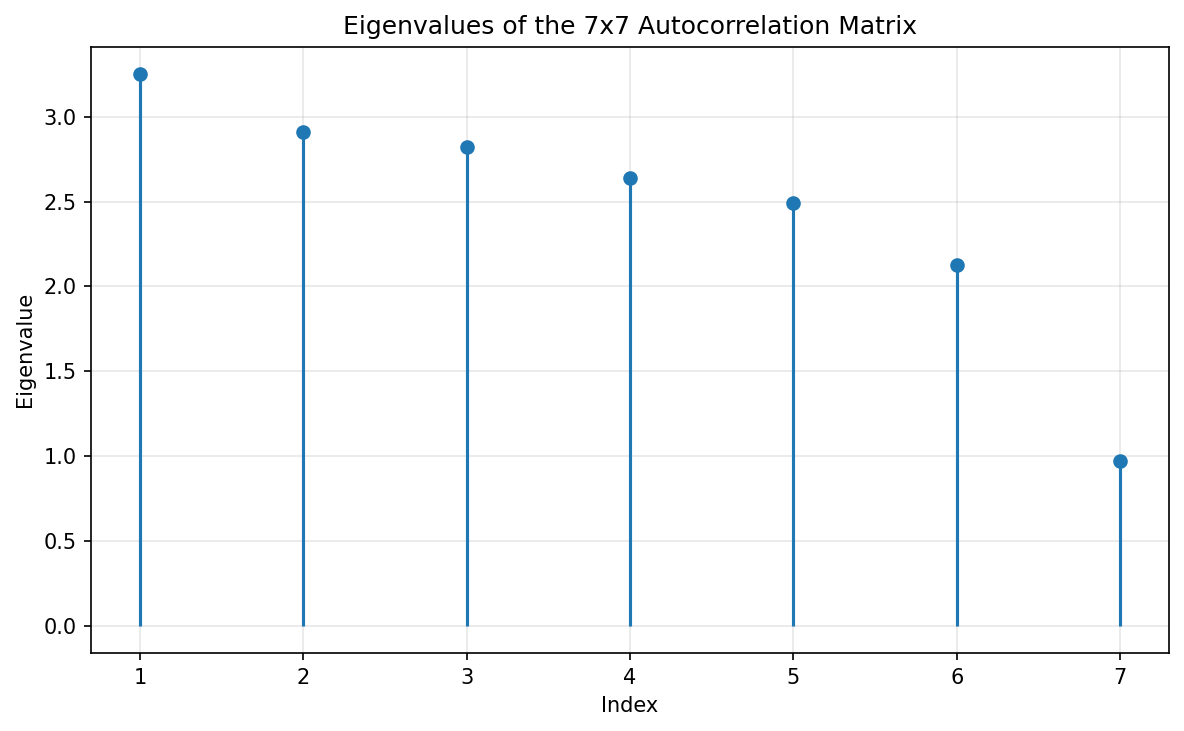
\includegraphics[width=0.72\textwidth]{lab01_fig08_acm_eigenvalues.png}
  \caption{Eigenvalues of the 7x7 autocorrelation matrix used for PHD and MUSIC.}
  \label{fig:eigs}
\end{figure}

Figure~\ref{fig:eigs} shows six large eigenvalues and one smaller eigenvalue, which is consistent with the model of six signal-space components and one noise-space component \cite{pisarenko1973}.

\section{Task 9: MUSIC Pseudo-Spectrum}
The MUSIC method partitions the autocorrelation matrix eigenvectors into signal and noise subspaces. With a 7x7 matrix and $p=6$, the noise subspace is one-dimensional. For a trial digital frequency $\omega$, the steering vector is
\begin{equation}
\mathbf{e}(\omega) =
\begin{bmatrix}
1 & e^{j\omega} & e^{j2\omega} & e^{j3\omega} & e^{j4\omega} & e^{j5\omega} & e^{j6\omega}
\end{bmatrix}^{T},
\end{equation}
and the MUSIC pseudo-spectrum is
\begin{equation}
P_{\mathrm{MUSIC}}(\omega) = \frac{1}{\left\| \mathbf{E}_{n}^{H}\mathbf{e}(\omega) \right\|^{2}}.
\end{equation}
The pseudo-spectrum generated from the verified code is shown in Fig.~\ref{fig:music}.
\begin{figure}[H]
  \centering
  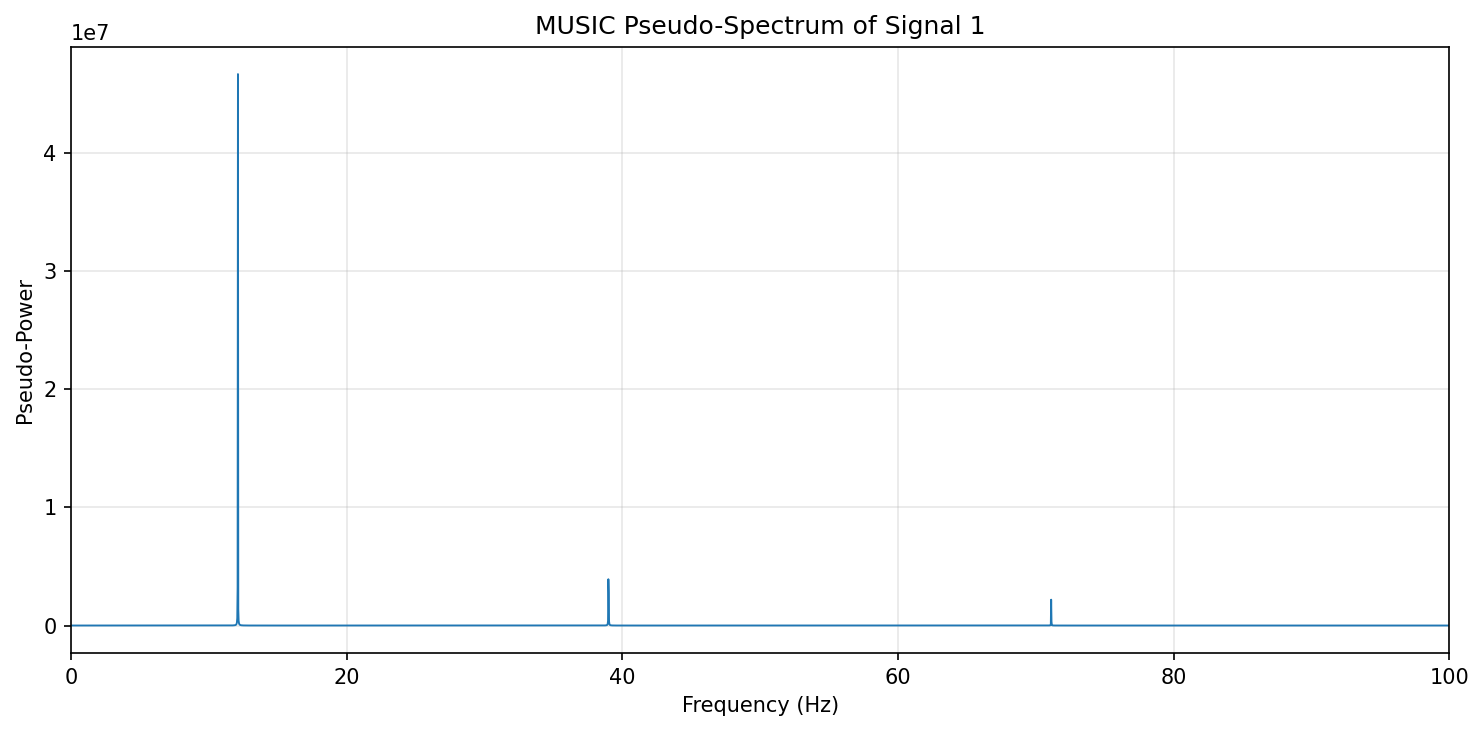
\includegraphics[width=0.86\textwidth]{lab01_fig09_music.png}
  \caption{MUSIC pseudo-spectrum of Signal 1.}
  \label{fig:music}
\end{figure}

The frequency estimates obtained from the dominant peaks of Fig.~\ref{fig:music} are listed in Table~\ref{tab:music}. The method is highly selective, with sharp peaks near the true frequencies even in the presence of noise \cite{schmidt1986, stoica2005}.
\begin{table}[H]
  \centering
  \caption{MUSIC frequency estimates for Signal 1.}
  \label{tab:music}
  \begin{tabular}{ccc}
    \toprule
    True Frequency (Hz) & Estimated Frequency (Hz) & Error (Hz) \\
    \midrule
    12.000 & 12.1030 & 0.1030 \\
    39.000 & 38.9847 & 0.0153 \\
    71.000 & 71.1178 & 0.1178 \\
    \bottomrule
  \end{tabular}
\end{table}

Compared with the DFT, MUSIC produces much narrower peaks because it uses a parametric subspace model rather than the finite-resolution Fourier grid alone. This makes it especially attractive for noisy data and for scenarios involving closely spaced spectral lines, provided that the model order is known or estimated reliably \cite{schmidt1986}.

\section{Task 10: Autoregressive Model}
The final task was to form an autoregressive model and examine its power spectrum. The linear prediction model solves
\begin{equation}
\hat{\boldsymbol{\theta}} = (\mathbf{A}^{T}\mathbf{A})^{-1}\mathbf{A}^{T}\mathbf{b},
\end{equation}
where $\mathbf{A}$ is the data matrix assembled from lagged samples and $\mathbf{b}$ contains the forward samples. The corresponding prediction polynomial is
\begin{equation}
V(z) = 1 - a_1 z^{-1} - a_2 z^{-2} - \cdots - a_N z^{-N},
\end{equation}
and the AR power spectrum is
\begin{equation}
P_{\mathrm{AR}}(\omega) = \left| \frac{1}{V(e^{j\omega})} \right|^2.
\end{equation}
The selected AR spectrum is shown in Fig.~\ref{fig:ar}.
\begin{figure}[H]
  \centering
  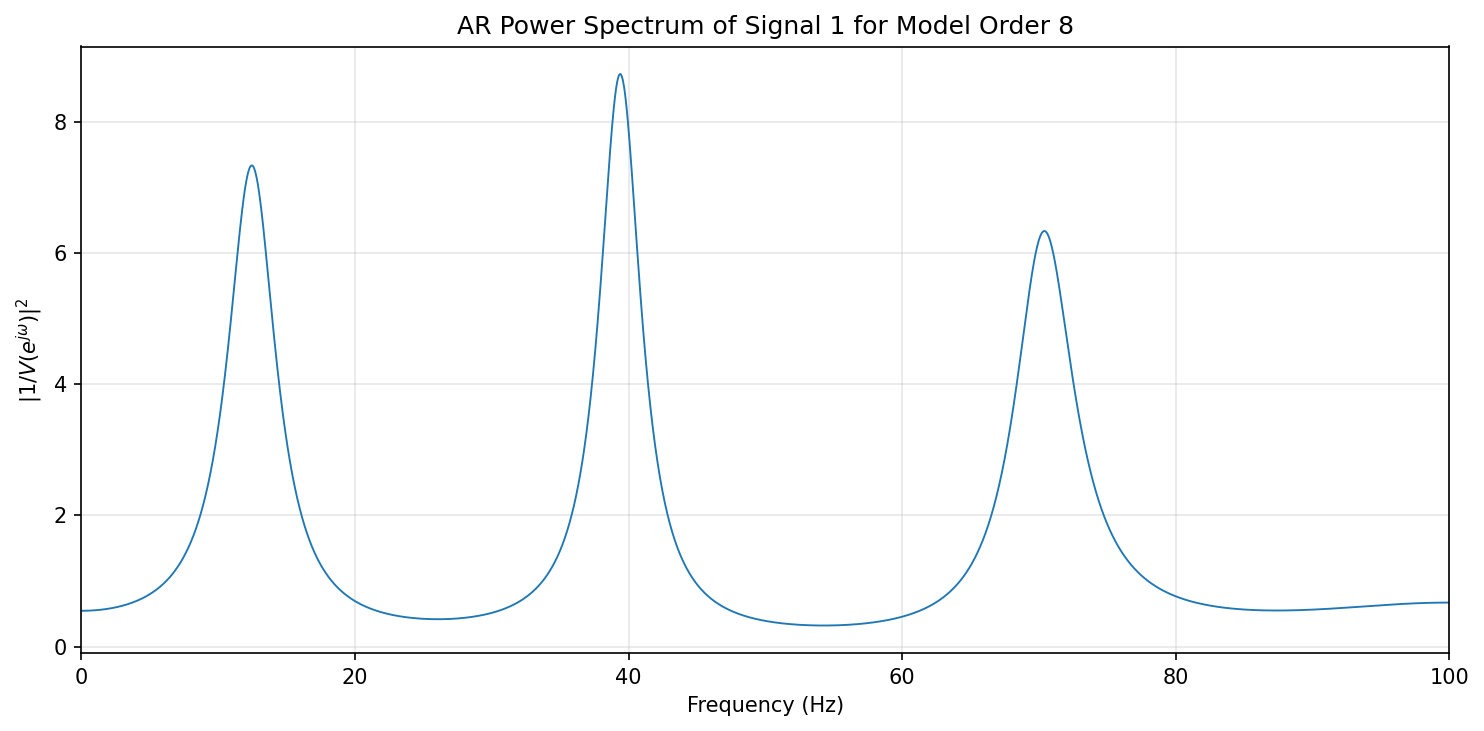
\includegraphics[width=0.86\textwidth]{lab01_fig10_ar.png}
  \caption{Least-squares AR spectrum of Signal 1 for model order 8.}
  \label{fig:ar}
\end{figure}

The eigenvalue separation in Fig.~\ref{fig:eigs} suggests a six-component signal space, but the smallest least-squares AR order that resolved all three tones robustly in this dataset was $N=8$. That slightly conservative order avoids under-modeling while remaining close to the autocorrelation-matrix elbow. The resulting frequency estimates are listed in Table~\ref{tab:ar}.
\begin{table}[H]
  \centering
  \caption{AR frequency estimates for Signal 1.}
  \label{tab:ar}
  \begin{tabular}{ccc}
    \toprule
    True Frequency (Hz) & Estimated Frequency (Hz) & Error (Hz) \\
    \midrule
    12.000 & 12.4500 & 0.4500 \\
    39.000 & 39.4000 & 0.4000 \\
    71.000 & 70.4000 & 0.6000 \\
    \bottomrule
  \end{tabular}
\end{table}

The AR model provides a sharper spectrum than the non-parametric DFT for a given display grid, but its quality depends strongly on the order selection. If the order is too small, peaks merge or disappear; if it is too large, spurious poles may appear \cite{akaike1974, stoica2005}. In this experiment, the AR estimator recovered all three tones but with larger bias than the DFT and MUSIC estimates.

\section{Conclusion}
This laboratory compared several complementary spectral estimators on a stationary multi-tone signal and a non-stationary chirp. The DFT provided highly accurate frequency estimates for Signal 1 because the record length was long enough to give a frequency spacing of approximately 0.01 Hz. However, it remained a global transform, so the chirp energy in Signal 2 was smeared over a range of frequencies. The spectrogram resolved that limitation by explicitly showing the stationary horizontal bands of Signal 1 and the time-varying diagonal trajectory of Signal 2.

Autocorrelation analysis was useful for periodicity interpretation rather than for direct frequency readout. For Signal 1, the exact common period is 1 s, yet the dominant short-lag periodicity was close to $1/12$ s because the 12 Hz component governs the most visible near-origin oscillation. The periodogram reframed the same information as spectral power, while MUSIC demonstrated the value of model-based super-resolution through sharp peaks near the true frequencies. The AR model also produced a concentrated spectrum, but its output depended noticeably on order selection.

From an engineering viewpoint, the results show that no single method is universally best. The DFT is simple and reliable, autocorrelation is valuable for periodicity and model construction, spectrograms are essential for non-stationary signals, MUSIC is powerful when the model order is known, and AR models offer compact parametric descriptions when order selection is handled carefully. These trade-offs are directly relevant in instrumentation, communications, vibration monitoring, and array processing applications.

\begin{thebibliography}{99}
\bibitem{oppenheim2010}
A. V. Oppenheim and R. W. Schafer, \textit{Discrete-Time Signal Processing}, 3rd ed. Upper Saddle River, NJ, USA: Prentice-Hall, 2010.

\bibitem{proakis2007}
J. G. Proakis and D. G. Manolakis, \textit{Digital Signal Processing: Principles, Algorithms, and Applications}, 4th ed. Upper Saddle River, NJ, USA: Prentice-Hall, 2007.

\bibitem{mitra2011}
S. K. Mitra, \textit{Digital Signal Processing: A Computer-Based Approach}, 4th ed. New York, NY, USA: McGraw-Hill, 2011.

\bibitem{welch1967}
P. D. Welch, ``The use of fast Fourier transform for the estimation of power spectra: A method based on time averaging over short, modified periodograms,'' \textit{IEEE Trans. Audio Electroacoust.}, vol. 15, no. 2, pp. 70--73, Jun. 1967.

\bibitem{schmidt1986}
R. O. Schmidt, ``Multiple emitter location and signal parameter estimation,'' \textit{IEEE Trans. Antennas Propag.}, vol. 34, no. 3, pp. 276--280, Mar. 1986.

\bibitem{pisarenko1973}
V. F. Pisarenko, ``The retrieval of harmonics from a covariance function,'' \textit{Geophys. J. Int.}, vol. 33, no. 3, pp. 347--366, Sep. 1973.

\bibitem{akaike1974}
H. Akaike, ``A new look at the statistical model identification,'' \textit{IEEE Trans. Autom. Control}, vol. 19, no. 6, pp. 716--723, Dec. 1974.

\bibitem{stoica2005}
P. Stoica and R. Moses, \textit{Spectral Analysis of Signals}. Upper Saddle River, NJ, USA: Prentice-Hall, 2005.
\end{thebibliography}

\appendix
\section{Python Source Code}

\subsection{Signal Construction and Time-Domain Analysis}
\begin{lstlisting}[caption={Imports, helper functions, signal construction, and time-domain plots for Lab 01.}, label={lst:lab01_time}]
import json
import math
from pathlib import Path

import matplotlib
matplotlib.use("Agg")
import matplotlib.pyplot as plt
import numpy as np
from scipy import signal
from scipy.fft import fft, fftfreq
from scipy.linalg import toeplitz


OUTPUT_DIR = Path(".")


def positive_lag_power_acf(x: np.ndarray) -> np.ndarray:
    """Return R[ell] for ell >= 0 using the lab-sheet power-signal estimator."""
    n_samples = len(x)
    full_corr = signal.correlate(x, x, mode="full", method="fft")
    positive_corr = full_corr[n_samples - 1 :]

    r = np.zeros(n_samples)
    for ell in range(n_samples):
        r[ell] = positive_corr[ell] / (n_samples - ell)
    return r


def full_power_acf_from_positive(r_positive: np.ndarray) -> np.ndarray:
    return np.concatenate((r_positive[1:][::-1], r_positive))


def one_sided_spectrum(x: np.ndarray, fs: float) -> tuple[np.ndarray, np.ndarray]:
    x_fft = fft(x)
    freqs = fftfreq(len(x), d=1.0 / fs)
    keep = freqs >= 0
    return freqs[keep], np.abs(x_fft[keep])


def top_peak_frequencies(freqs: np.ndarray, magnitude: np.ndarray, count: int) -> list[float]:
    distance = max(1, len(freqs) // 400)
    peaks, properties = signal.find_peaks(magnitude, distance=distance)
    if len(peaks) == 0:
        return []
    order = np.argsort(properties.get("peak_heights", magnitude[peaks]))[::-1]
    ranked = peaks[order]
    selected = []
    for idx in ranked:
        freq_hz = float(freqs[idx])
        if any(abs(freq_hz - prev) < 0.5 for prev in selected):
            continue
        selected.append(freq_hz)
        if len(selected) == count:
            break
    return sorted(selected)


def local_peak_near_expected(
    lags_seconds: np.ndarray,
    acf_positive: np.ndarray,
    expected_period: float,
    search_half_width: float,
) -> float:
    mask = np.logical_and(
        lags_seconds >= expected_period - search_half_width,
        lags_seconds <= expected_period + search_half_width,
    )
    if not np.any(mask):
        return float(expected_period)
    sub_lags = lags_seconds[mask]
    sub_acf = acf_positive[mask]
    idx = int(np.argmax(sub_acf))
    return float(sub_lags[idx])


def ar_least_squares_coefficients(x: np.ndarray, order: int) -> np.ndarray:
    rows = len(x) - order
    a_matrix = np.zeros((rows, order))
    b_vector = x[order:]
    for col in range(order):
        a_matrix[:, col] = x[order - col - 1 : len(x) - col - 1]
    theta_hat, *_ = np.linalg.lstsq(a_matrix, b_vector, rcond=None)
    return theta_hat


def save_figure(filename: str) -> None:
    plt.savefig(OUTPUT_DIR / filename, dpi=150, bbox_inches="tight")
    plt.close("all")


def main() -> None:
    np.random.seed(291)

    a, b, c = 2, 9, 1
    f1 = 10 + a
    f2 = 30 + b
    f3 = 70 + c
    fs = 200.0
    duration = 100.0
    t = np.linspace(0.0, duration, int(duration * fs) + 1)
    n_samples = len(t)
    noise = np.random.randn(n_samples)

    signal_1 = (
        np.sin(2.0 * np.pi * f1 * t)
        + np.cos(2.0 * np.pi * f2 * t)
        + np.sin(2.0 * np.pi * f3 * t)
        + noise
    )
    signal_2 = np.sin(20.0 * np.pi * t + 2.0 * np.pi * (t**2 / 150.0)) + noise

    time_mask = t <= 2.0
    plt.figure(figsize=(10, 7))
    plt.subplot(2, 1, 1)
    plt.plot(t[time_mask], signal_1[time_mask], linewidth=0.9)
    plt.title("Signal 1 in the Time Domain (First 2 s)")
    plt.xlabel("Time (s)")
    plt.ylabel("Amplitude")
    plt.grid(True, alpha=0.3)
    plt.subplot(2, 1, 2)
    plt.plot(t[time_mask], signal_2[time_mask], linewidth=0.9, color="tab:orange")
    plt.title("Signal 2 in the Time Domain (First 2 s)")
    plt.xlabel("Time (s)")
    plt.ylabel("Amplitude")
    plt.grid(True, alpha=0.3)
    plt.tight_layout()
    save_figure("lab01_fig01_signals.png")

    plt.figure(figsize=(10, 7))
    plt.subplot(2, 1, 1)
    plt.hist(signal_1, bins=60, color="steelblue", edgecolor="black")
    plt.title("Histogram of Signal 1")
    plt.xlabel("Amplitude")
    plt.ylabel("Count")
    plt.subplot(2, 1, 2)
    plt.hist(signal_2, bins=60, color="darkseagreen", edgecolor="black")
    plt.title("Histogram of Signal 2")
    plt.xlabel("Amplitude")
    plt.ylabel("Count")
    plt.tight_layout()
    save_figure("lab01_fig02_histograms.png")
\end{lstlisting}

\subsection{Discrete Fourier Transform Analysis}
\begin{lstlisting}[caption={DFT computation and peak extraction for Lab 01.}, label={lst:lab01_dft}]
    freqs_1, dft_mag_1 = one_sided_spectrum(signal_1, fs)
    freqs_2, dft_mag_2 = one_sided_spectrum(signal_2, fs)
    dft_estimates = top_peak_frequencies(freqs_1, dft_mag_1, 3)

    plt.figure(figsize=(10, 7))
    plt.subplot(2, 1, 1)
    plt.plot(freqs_1, dft_mag_1, linewidth=0.8)
    plt.title("One-Sided DFT Magnitude of Signal 1")
    plt.xlabel("Frequency (Hz)")
    plt.ylabel(r"$|X_1[k]|$")
    plt.xlim(0.0, fs / 2.0)
    plt.grid(True, alpha=0.3)
    plt.subplot(2, 1, 2)
    plt.plot(freqs_2, dft_mag_2, linewidth=0.8, color="tab:orange")
    plt.title("One-Sided DFT Magnitude of Signal 2")
    plt.xlabel("Frequency (Hz)")
    plt.ylabel(r"$|X_2[k]|$")
    plt.xlim(0.0, fs / 2.0)
    plt.grid(True, alpha=0.3)
    plt.tight_layout()
    save_figure("lab01_fig03_dft.png")
\end{lstlisting}

\subsection{Spectrogram Analysis}
\begin{lstlisting}[caption={Spectrogram analysis for both Lab 01 signals.}, label={lst:lab01_spec}]
    nperseg = 512
    noverlap = 384
    spec_f1, spec_t1, spec_s1 = signal.spectrogram(
        signal_1, fs=fs, nperseg=nperseg, noverlap=noverlap, scaling="density"
    )
    spec_f2, spec_t2, spec_s2 = signal.spectrogram(
        signal_2, fs=fs, nperseg=nperseg, noverlap=noverlap, scaling="density"
    )

    plt.figure(figsize=(10, 8))
    plt.subplot(2, 1, 1)
    plt.pcolormesh(spec_t1, spec_f1, 10.0 * np.log10(spec_s1 + 1e-12), shading="auto")
    plt.title("Spectrogram of Signal 1")
    plt.ylabel("Frequency (Hz)")
    plt.colorbar(label="Power/Frequency (dB/Hz)")
    plt.subplot(2, 1, 2)
    plt.pcolormesh(spec_t2, spec_f2, 10.0 * np.log10(spec_s2 + 1e-12), shading="auto")
    plt.title("Spectrogram of Signal 2")
    plt.xlabel("Time (s)")
    plt.ylabel("Frequency (Hz)")
    plt.colorbar(label="Power/Frequency (dB/Hz)")
    plt.tight_layout()
    save_figure("lab01_fig04_spectrogram.png")
\end{lstlisting}

\subsection{Autocorrelation Function}
\begin{lstlisting}[caption={Autocorrelation estimators for Signal 1 and Signal 2.}, label={lst:lab01_acf}]
    acf_builtin_s1 = signal.correlate(signal_1, signal_1, mode="full", method="fft") / n_samples
    acf_positive_s1 = positive_lag_power_acf(signal_1)
    acf_manual_s1 = full_power_acf_from_positive(acf_positive_s1)

    acf_builtin_s2 = signal.correlate(signal_2, signal_2, mode="full", method="fft") / n_samples
    acf_positive_s2 = positive_lag_power_acf(signal_2)
    acf_manual_s2 = full_power_acf_from_positive(acf_positive_s2)

    lags = signal.correlation_lags(n_samples, n_samples)
    lags_seconds = lags / fs
    positive_lags_seconds = np.arange(n_samples) / fs
    zoom_mask = np.logical_and(lags_seconds >= 0.0, lags_seconds <= 1.5)

    dominant_period_s1 = local_peak_near_expected(
        positive_lags_seconds[1:],
        acf_positive_s1[1:],
        expected_period=1.0 / f1,
        search_half_width=0.01,
    )
    common_period_exact = 1.0 / math.gcd(math.gcd(f1, f2), f3)

    plt.figure(figsize=(10, 7))
    plt.subplot(2, 1, 1)
    plt.plot(lags_seconds[zoom_mask], acf_builtin_s1[zoom_mask], linewidth=0.9)
    plt.axvline(dominant_period_s1, color="tab:red", linestyle="--", label="Dominant visible peak")
    plt.title("Signal 1 Autocorrelation Using scipy.signal.correlate")
    plt.xlabel("Lag (s)")
    plt.ylabel(r"$\hat{r}_{xx}[\ell]$")
    plt.grid(True, alpha=0.3)
    plt.legend()
    plt.subplot(2, 1, 2)
    plt.plot(lags_seconds[zoom_mask], acf_manual_s1[zoom_mask], linewidth=0.9, color="tab:green")
    plt.axvline(dominant_period_s1, color="tab:red", linestyle="--", label="Dominant visible peak")
    plt.title("Signal 1 Autocorrelation Using the Power-Signal Estimator")
    plt.xlabel("Lag (s)")
    plt.ylabel(r"$\hat{r}_{xx}[\ell]$")
    plt.grid(True, alpha=0.3)
    plt.legend()
    plt.tight_layout()
    save_figure("lab01_fig05_autocorr_s1.png")

    plt.figure(figsize=(10, 7))
    plt.subplot(2, 1, 1)
    plt.plot(lags_seconds[zoom_mask], acf_builtin_s2[zoom_mask], linewidth=0.9)
    plt.title("Signal 2 Autocorrelation Using scipy.signal.correlate")
    plt.xlabel("Lag (s)")
    plt.ylabel(r"$\hat{r}_{xx}[\ell]$")
    plt.grid(True, alpha=0.3)
    plt.subplot(2, 1, 2)
    plt.plot(lags_seconds[zoom_mask], acf_manual_s2[zoom_mask], linewidth=0.9, color="tab:green")
    plt.title("Signal 2 Autocorrelation Using the Power-Signal Estimator")
    plt.xlabel("Lag (s)")
    plt.ylabel(r"$\hat{r}_{xx}[\ell]$")
    plt.grid(True, alpha=0.3)
    plt.tight_layout()
    save_figure("lab01_fig06_autocorr_s2.png")
\end{lstlisting}

\subsection{Periodogram}
\begin{lstlisting}[caption={Periodogram formation from the FFT of the full autocorrelation sequence.}, label={lst:lab01_periodogram}]
    periodogram_s1 = np.abs(fft(np.fft.ifftshift(acf_builtin_s1)))
    periodogram_s2 = np.abs(fft(np.fft.ifftshift(acf_builtin_s2)))
    periodogram_freqs = fftfreq(len(acf_builtin_s1), d=1.0 / fs)
    periodogram_mask = periodogram_freqs >= 0.0

    plt.figure(figsize=(10, 7))
    plt.subplot(2, 1, 1)
    plt.plot(periodogram_freqs[periodogram_mask], periodogram_s1[periodogram_mask], linewidth=0.8)
    plt.title("Periodogram of Signal 1 from the FFT of the Full Autocorrelation")
    plt.xlabel("Frequency (Hz)")
    plt.ylabel("Power")
    plt.xlim(0.0, fs / 2.0)
    plt.grid(True, alpha=0.3)
    plt.subplot(2, 1, 2)
    plt.plot(
        periodogram_freqs[periodogram_mask],
        periodogram_s2[periodogram_mask],
        linewidth=0.8,
        color="tab:orange",
    )
    plt.title("Periodogram of Signal 2 from the FFT of the Full Autocorrelation")
    plt.xlabel("Frequency (Hz)")
    plt.ylabel("Power")
    plt.xlim(0.0, fs / 2.0)
    plt.grid(True, alpha=0.3)
    plt.tight_layout()
    save_figure("lab01_fig07_periodogram.png")
\end{lstlisting}

\subsection{MUSIC Pseudo-Spectrum}
\begin{lstlisting}[caption={Autocorrelation matrix construction, eigenanalysis, and MUSIC pseudo-spectrum generation.}, label={lst:lab01_music}]
    p_components = 6
    acm_size = p_components + 1
    acm = toeplitz(acf_positive_s1[:acm_size])
    eigenvalues, eigenvectors = np.linalg.eigh(acm)
    sort_idx = np.argsort(eigenvalues)[::-1]
    eigenvalues_desc = eigenvalues[sort_idx]
    eigenvectors_desc = eigenvectors[:, sort_idx]

    plt.figure(figsize=(8, 5))
    plt.stem(np.arange(1, acm_size + 1), eigenvalues_desc, basefmt=" ")
    plt.title("Eigenvalues of the 7x7 Autocorrelation Matrix")
    plt.xlabel("Index")
    plt.ylabel("Eigenvalue")
    plt.grid(True, alpha=0.3)
    plt.tight_layout()
    save_figure("lab01_fig08_acm_eigenvalues.png")

    e_noise = eigenvectors_desc[:, -1:]
    music_freqs = np.linspace(0.0, fs / 2.0, 4000)
    music_spectrum = np.zeros_like(music_freqs)
    for idx, freq_hz in enumerate(music_freqs):
        omega = 2.0 * np.pi * freq_hz / fs
        steering = np.exp(1j * omega * np.arange(acm_size))[:, None]
        projection = e_noise.conj().T @ steering
        music_spectrum[idx] = 1.0 / np.linalg.norm(projection) ** 2
    music_estimates = top_peak_frequencies(music_freqs, music_spectrum, 3)

    plt.figure(figsize=(10, 5))
    plt.plot(music_freqs, music_spectrum, linewidth=0.9)
    plt.title("MUSIC Pseudo-Spectrum of Signal 1")
    plt.xlabel("Frequency (Hz)")
    plt.ylabel("Pseudo-Power")
    plt.xlim(0.0, fs / 2.0)
    plt.grid(True, alpha=0.3)
    plt.tight_layout()
    save_figure("lab01_fig09_music.png")
\end{lstlisting}

\subsection{Autoregressive Model}
\begin{lstlisting}[caption={Least-squares AR model, AR spectrum, and result export for Lab 01.}, label={lst:lab01_ar}]
    ar_order = 8
    theta_hat = ar_least_squares_coefficients(signal_1, ar_order)
    ar_den = np.concatenate(([1.0], -theta_hat))
    ar_freqs, ar_response = signal.freqz([1.0], ar_den, worN=4000, fs=fs)
    ar_spectrum = np.abs(ar_response) ** 2
    ar_estimates = top_peak_frequencies(ar_freqs, ar_spectrum, 3)

    plt.figure(figsize=(10, 5))
    plt.plot(ar_freqs, ar_spectrum, linewidth=0.9)
    plt.title(f"AR Power Spectrum of Signal 1 for Model Order {ar_order}")
    plt.xlabel("Frequency (Hz)")
    plt.ylabel(r"$|1/V(e^{j\omega})|^2$")
    plt.xlim(0.0, fs / 2.0)
    plt.grid(True, alpha=0.3)
    plt.tight_layout()
    save_figure("lab01_fig10_ar.png")

    results = {
        "student": {"e_number": "E/21/291", "a": a, "b": b, "c": c},
        "signal_parameters": {
            "f1_hz": f1,
            "f2_hz": f2,
            "f3_hz": f3,
            "fs_hz": fs,
            "duration_s": duration,
            "n_samples": n_samples,
            "frequency_resolution_hz": fs / n_samples,
            "spectrogram_nperseg": nperseg,
            "spectrogram_noverlap": noverlap,
        },
        "task_3_dft_estimates_hz": dft_estimates,
        "task_5_signal_1": {
            "dominant_visible_period_s": dominant_period_s1,
            "exact_common_period_s": common_period_exact,
        },
        "task_7_periodogram_peak_estimates_hz": top_peak_frequencies(
            periodogram_freqs[periodogram_mask], periodogram_s1[periodogram_mask], 3
        ),
        "task_8": {
            "p": p_components,
            "acm_size": acm_size,
            "eigenvalues_desc": [float(value) for value in eigenvalues_desc],
        },
        "task_9_music_estimates_hz": music_estimates,
        "task_10_ar": {
            "model_order": ar_order,
            "estimated_frequencies_hz": ar_estimates,
            "selection_note": "Order 8 was chosen as the smallest least-squares AR model that resolved all three tones while remaining close to the ACM eigenvalue elbow at six signal components.",
            "theta_hat": [float(value) for value in theta_hat],
        },
    }

    with open(OUTPUT_DIR / "lab01_results.json", "w", encoding="utf-8") as file:
        json.dump(results, file, indent=2)

    print(json.dumps(results, indent=2))


if __name__ == "__main__":
    main()
\end{lstlisting}

\end{document}
